% !TeX program = lualatex
% !TeX encoding = utf8
% !TeX spellcheck = uk_UA
% !BIB program = bibler

\documentclass[onlytextwidth]{beamer}
\usetheme{Electromagnetism}
\usepackage{emf}

\usepackage{Electromagnetism}
\usepackage{circuitikz}
\usepackage{pgfplots}
\pgfplotsset{compat=1.17}
\usetikzlibrary{arrows.meta,calc}
\hypersetup{
  colorlinks=true,
  linkcolor=cyan,  % Цвет для внутренних ссылок
  urlcolor=red,    % Цвет для URL
  citecolor=blue   % Цвет для библиографических ссылок
}




%============================================================================
\title[Лекції електрики та магнетизму]{\huge\bfseries Коливальні процеси \\ в електричних колах}
\subtitle{Лекції з електрики та магнетизму}
\author{Пономаренко С. М.}
\date{}
%============================================================================
\graphicspath{{pictures/}}
\begin{document}


\begin{frame}[plain]
	\maketitle
\end{frame}

% ============================== Слайд ## ===================================
\begin{frame}{Зміст лекції}{}
	\tableofcontents
\end{frame}
% ===========================================================================

%% --------------------------------------------------------
\section{Квазістаціонарне наближення}
%% --------------------------------------------------------

% ============================== Слайд ## ===================================
\begin{frame}{Квазістаціонарне наближення}{}
	\begin{block}{}\justifying
		Процес --- \alert{квазістаціонарний}, якщо миттєві значення струму в усіх ділянках нерозгалуженого кола однакові, а поля в конденсаторах такі самі, як в електростатиці.
	\end{block}
	\begin{block}{}\justifying
		Якщо частота сигналу $\omega$, довжина хвилі $\lambda = cT$, довжина кола $l$, а час поширення сигналу по колу $\tau \sim l/c$, то умова квазістаціонарності:
		\begin{equation*}
			\tcbhighmath{
				l \ll \lambda \qquad\Leftrightarrow\qquad \tau \ll T.
			}
		\end{equation*}
	\end{block}
	\begin{exampleblock}{}\justifying\small
		Для мережі 50 Гц $\lambda \approx 6000$ км --- запас у сотні тисяч разів; для довгої ЛЕП це вже помітна частка $\lambda$, і просту схему $R,L,C$ доводиться заміняти теорією довгих ліній. Далі коло описуємо як систему із \alert{зосередженими} елементами $R$, $L$, $C$ --- у цьому наближенні чинні закон Ома, правила Кірхгофа та рівняння коливального контуру.
	\end{exampleblock}
\end{frame}
% ===========================================================================

%% --------------------------------------------------------
\section{Вільні коливання в коливальному контурі}
%% --------------------------------------------------------

% ============================== Слайд ## ===================================
\begin{frame}{Рівняння коливального контуру}{}
	\begin{columns}
		\begin{column}{0.48\linewidth}\centering
			\begin{circuitikz}[european resistors, scale=0.85, thick]
				\coordinate (A) at (0,0);
				\coordinate (B) at (4,0);
				\coordinate (C) at (4,3);
				\coordinate (D) at (0,3);
				\coordinate (T1) at ($(A)!0.4!(B)$);
				\coordinate (T2) at ($(A)!0.6!(B)$);
				\draw (A) to[short, -o] (T1) node[above] {1};
				\draw (B) to[short, -o] (T2) node[above] {2};
				\path (T1) -- (T2) node[midway, below=2pt] {$\emf$};
				\draw (B) to[L, mirror, l_=$L$] (C);
				\draw (C) to[R, l_=$R$] (D);
				\draw[->, >=latex] ($(C)!0.325!(D) + (0,-0.5)$) -- ($(C)!0.675!(D) + (0,-0.5)$)
				node[midway, below] {$J$};
				\draw (D) to[C, l_=$C$] (A);
				\node at ($(D)!0.4!(A) + (0.3,0)$) {3};
				\node at ($(D)!0.6!(A) + (0.3,0)$) {4};
				\node at ($(D)!0.3!(A) + (-0.4,0)$) {$+q$};
				\node at ($(D)!0.7!(A) + (-0.4,0)$) {$-q$};
			\end{circuitikz}
		\end{column}
		\begin{column}{0.52\linewidth}\justifying\small
			За теоремою про циркуляцію для контуру $\{12341\}$:
			\begin{equation*}
				\oint E_l\,dl = -\frac{d\Phi}{dt}, \qquad \Phi = LJ.
			\end{equation*}
			Ділянки: $12$ --- ЕРС ($\emf=\varphi_2-\varphi_1$), $23$ --- опір ($JR$), $34$ --- конденсатор ($q/C$), $41$ --- без елементів.
		\end{column}
	\end{columns}
	\begin{block}{}\justifying
		Рівняння коливального контуру:
		\begin{equation*}
			\tcbhighmath{
				L\frac{dJ}{dt} + JR + \frac{q}{C} = \emf.
			}
		\end{equation*}
	\end{block}
\end{frame}
% ===========================================================================

% ============================== Слайд ## ===================================
\begin{frame}{Вільні та гармонічні коливання}{}
	\begin{block}{}\justifying
		При $\emf=0$, з позначеннями $2\gamma = R/L$, $\omega_0^2 = 1/LC$ (і $J=\dot q$) рівняння коливального контуру набирає вигляду \alert{рівняння вільних коливань}:
		\begin{equation*}
			\tcbhighmath{
				\ddot q + 2\gamma\dot q + \omega_0^2 q = 0.
			}
		\end{equation*}
	\end{block}
	\begin{exampleblock}{}\justifying
		При $R=0$ ($\gamma=0$) --- рівняння гармонічного осцилятора, розв'язок
		\begin{equation*}
			q(t) = q_0\cos(\omega_0 t + \varphi_0), \qquad
			\tcbhighmath{
				T = \frac{2\pi}{\omega_0} = 2\pi\sqrt{LC}
			}
			\quad\text{(формула Томсона)}.
		\end{equation*}
		$q_0$ --- амплітуда, $\varphi = \omega_0 t + \varphi_0$ --- фаза коливань.
	\end{exampleblock}
\end{frame}
% ===========================================================================

% ============================== Слайд ## ===================================
\begin{frame}{Згасаючі коливання}{}
	\framesubtitle<1>{Слабке затухання $\omega_0 > \gamma$}
	\framesubtitle<2>{Сильне затухання $\omega_0 < \gamma$}
	\framesubtitle<3>{Критичне затухання $\omega_0 = \gamma$}
	\begin{block}{}\justifying\small
		Шукаємо комплексний розв'язок $\hat q(t) = q_0 e^{i\Omega t}$; корені характеристичного рівняння $\Omega_{1,2} = i\gamma \pm \sqrt{\omega_0^2-\gamma^2}$, а $q(t) = \operatorname{Re}\hat q(t)$.
	\end{block}
	\begin{overprint}
		\onslide<1>
		\begin{columns}
			\begin{column}{0.5\linewidth}\justifying
				Позначимо $\omega = \sqrt{\omega_0^2-\gamma^2}$:
				\begin{equation*}
					\tcbhighmath{
						q(t) = q_0 e^{-\gamma t}\cos(\omega t + \varphi_0).
					}
				\end{equation*}
				$\gamma$ --- \alert{коефіцієнт затухання}, $\tau = 1/\gamma$ --- \alert{час затухання} (амплітуда спадає в $e$ разів).
			\end{column}
			\begin{column}{0.5\linewidth}\centering
				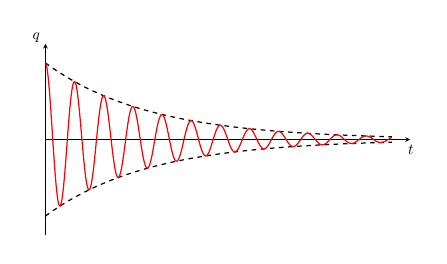
\begin{tikzpicture}[scale=0.55]
					\begin{axis}[
							axis lines=center, xlabel={$t$}, ylabel={$q$},
							x label style={anchor=north west, at={(axis description cs:0.98,0.5)}},
							y label style={anchor=south east, at={(axis description cs:0,0.98)}},
							xmin=0, xmax=10, ymin=-1.25, ymax=1.25, ticks=none,
							width=10cm, height=6cm, samples=500
						]
						\addplot [dashed, domain=0:9.5, thick] {exp(-0.35*x)};
						\addplot [dashed, domain=0:9.5, thick] {-exp(-0.35*x)};
						\addplot [red, thick, domain=0:9.5] {exp(-0.35*x) * cos(deg(2.5*pi*x))};
					\end{axis}
				\end{tikzpicture}
			\end{column}
		\end{columns}
		\onslide<2>
		\begin{block}{}\justifying
			Позначимо $\Gamma = \sqrt{\gamma^2-\omega_0^2}$ --- розв'язок неперіодичний (аперіодичний):
			\begin{equation*}
				\tcbhighmath{
					q(t) = e^{-\gamma t}\left[q_{10}e^{\Gamma t} + q_{20}e^{-\Gamma t}\right].
				}
			\end{equation*}
		\end{block}
		\onslide<3>
		\begin{block}{}\justifying
			Корені збігаються ($\Omega_1=\Omega_2$), розв'язок вироджується:
			\begin{equation*}
				\tcbhighmath{
					q(t) = e^{-\gamma t}\left(C_1 + C_2 t\right).
				}
			\end{equation*}
		\end{block}
	\end{overprint}
\end{frame}
% ===========================================================================

% ============================== Слайд ## ===================================
\begin{frame}{Закон збереження енергії}{}
	\begin{block}{}\justifying
		Множимо рівняння $L\ddot q + q/C = -R\dot q$ на $\dot q = J$, враховуючи $\dot q\ddot q = \frac{d}{dt}\left(\tfrac12\dot q^2\right)$:
		\begin{equation*}
			\tcbhighmath{
				\frac{d}{dt}\left(\frac{LJ^2}{2} + \frac{q^2}{2C}\right) = -RJ^2.
			}
		\end{equation*}
	\end{block}
	\begin{block}{}\justifying
		Повна енергія контуру $W = W_L + W_C$, де $W_L = LJ^2/2$ (в котушці), $W_C = q^2/2C$ (в конденсаторі). Права частина ($-N=-RJ^2$) --- джоулеві втрати:
		\begin{equation*}
			\tcbhighmath{
				\frac{dW}{dt} = -N.
			}
		\end{equation*}
	\end{block}
\end{frame}
% ===========================================================================

% ============================== Слайд ## ===================================
\begin{frame}{Енергія в контурі без втрат}{}
	\begin{block}{}\justifying
		При $R=0$ ($N=0$) енергія зберігається:
		\begin{equation*}
			q(t) = q_0\cos\omega_0 t, \qquad J(t) = J_0\cos\!\left(\omega_0 t + \frac\pi2\right), \qquad J_0=\omega_0 q_0.
		\end{equation*}
		Фази $q(t)$ і $J(t)$ зсунуті на $\pi/2$.
	\end{block}
	\begin{block}{}\justifying
		$W_L$ і $W_C$ коливаються з однаковою амплітудою в \alert{протифазі}, а сума стала:
		\begin{equation*}
			\tcbhighmath{
				W_L + W_C = \frac{LJ_0^2}{2} + \frac{q_0^2}{2C} = \const.
			}
		\end{equation*}
	\end{block}
	\begin{exampleblock}{}\justifying\small
		При $R\ne0$ найбільші втрати --- у моменти максимального струму (максимальні джоулеві втрати $N=RJ^2$).
	\end{exampleblock}
\end{frame}
% ===========================================================================

% ============================== Слайд ## ===================================
\begin{frame}{Логарифмічний декремент і добротність}{}
	\begin{block}{}\justifying
		Для двох сусідніх максимумів $q_n$, $q_{n+1}$ \alert{логарифмічний декремент згасання}:
		\begin{equation*}
			\tcbhighmath{
				\delta = \ln(q_n/q_{n+1}) = \gamma T = \frac{2\pi\gamma}{\omega}.
			}
		\end{equation*}
		За час затухання $\tau=1/\gamma$ відбувається $n = 1/(\gamma T) = 1/\delta$ коливань.
	\end{block}
	\begin{block}{}\justifying
		\alert{Добротність} $Q = \pi n = \omega/2\gamma = \pi/\delta$; для послідовного $LCR$-контуру:
		\begin{equation*}
			\tcbhighmath{
				Q = \frac1R\sqrt{\frac LC}.
			}
		\end{equation*}
		Енергетичний сенс: за період втрачається $\Delta W = 2\gamma T\cdot W$, звідки
		\begin{equation*}
			\tcbhighmath{
				Q = 2\pi\frac{W}{\Delta W}.
			}
		\end{equation*}
	\end{block}
	\begin{exampleblock}{}\justifying\small
		$Q$ показує, скільки коливань система встигне зробити до втрати енергії: звичайний $LC$-контур --- десятки-сотні, кварцовий резонатор --- $10^4$--$10^6$, надпровідний резонатор прискорювача --- $10^9$--$10^{11}$.
	\end{exampleblock}
\end{frame}
% ===========================================================================

%% --------------------------------------------------------
\section{Вимушені коливання під дією гармонічної ЕРС}
%% --------------------------------------------------------

% ============================== Слайд ## ===================================
\begin{frame}{Рівняння вимушених коливань}{}
	\begin{block}{}\justifying
		Для $LCR$-контуру з гармонічною ЕРС $\emf(t)=\emf_0\cos\omega t$, переходячи до напруги $V=q/C$:
		\begin{equation*}
			\tcbhighmath{
				\ddot V + 2\gamma\dot V + \omega_0^2 V = \omega_0^2\emf_0\cos\omega t.
			}
		\end{equation*}
	\end{block}
	\begin{block}{}\justifying
		Загальний розв'язок $\hat V = \hat V_s + \hat V_f$: вільні коливання $\hat V_s$ згасають з часом ($\gamma\ne0$), залишаються тільки \alert{вимушені} коливання $\hat V_f(t) = \hat V_0 e^{i\omega t}$.
	\end{block}
\end{frame}
% ===========================================================================

% ============================== Слайд ## ===================================
\begin{frame}{Метод комплексних амплітуд}{}
	\begin{exampleblock}{}\justifying
		Для дійсної $x(t)=x_0\cos(\omega t+\varphi_0)$ вводимо комплексну функцію $z(t)=z_0e^{i\omega t}$ таку, що $x(t)=\operatorname{Re}z(t)$. Величина
		\begin{equation*}
			\tcbhighmath{
				z_0 = x_0e^{i\varphi_0}
			}
		\end{equation*}
		називається \alert{комплексною амплітудою}: її модуль --- амплітуда $x_0$, а фаза --- початкова фаза $\varphi_0$.
	\end{exampleblock}
	\begin{block}{}\justifying\small
		Формула Ейлера $e^{i\phi}=\cos\phi+i\sin\phi$ пов'язує гармонічні й експоненційні функції --- з останніми значно легше диференціювати й інтегрувати.
	\end{block}
\end{frame}
% ===========================================================================

% ============================== Слайд ## ===================================
\begin{frame}{Частотна характеристика. Резонанс}{}
	\begin{columns}
		\begin{column}{0.54\linewidth}\justifying\small
			\begin{equation*}
				\tcbhighmath{
					\hat V_0 = \frac{\omega_0^2\emf_0}{\omega_0^2-\omega^2+2i\gamma\omega}.
				}
			\end{equation*}
			\begin{equation*}
				V_f = V_0\cos(\omega t+\varphi_0), \quad
				V_0 = \frac{\omega_0^2\emf_0}{\sqrt{(\omega_0^2-\omega^2)^2+4\gamma^2\omega^2}}.
			\end{equation*}
			Різке зростання $V_0$ біля $\omega\approx\omega_0$ --- \alert{резонанс}; резонансна частота:
			\begin{equation*}
				\tcbhighmath{
					\omega_m = \sqrt{\omega_0^2-2\gamma^2}.
				}
			\end{equation*}
			При $\gamma\ge\omega_0/\sqrt2$ резонансу немає.
		\end{column}
		\begin{column}{0.46\linewidth}\centering
			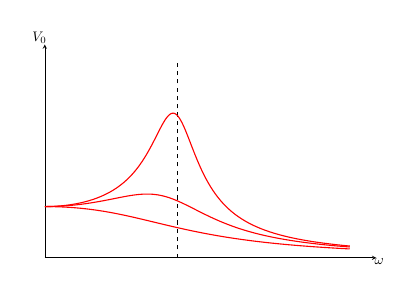
\begin{tikzpicture}[scale=0.5]
				\begin{axis}[
						axis lines=center, xlabel={$\omega$}, ylabel={$V_0$},
						x label style={anchor=north west, at={(axis description cs:0.98,0.02)}},
						y label style={anchor=south east, at={(axis description cs:0.02,0.98)}},
						xmin=0, xmax=2.5, ymin=0, ymax=2.5, ticks=none,
						width=10cm, height=7cm, samples=400
					]
					\draw[dashed, thick] (axis cs:1.0,0) -- (axis cs:1.0,2.3);
					\node[below=2pt] at (axis cs:1.0,0) {$\omega_0$};
					\addplot [red, thick, domain=0:2.3] {0.6 / sqrt((1 - x^2)^2 + 4*(0.18^2)*x^2)};
					\addplot [red, thick, domain=0:2.3] {0.6 / sqrt((1 - x^2)^2 + 4*(0.45^2)*x^2)};
					\addplot [red, thick, domain=0:2.3] {0.6 / sqrt((1 - x^2)^2 + 4*(0.85^2)*x^2)};
				\end{axis}
			\end{tikzpicture}
		\end{column}
	\end{columns}
\end{frame}
% ===========================================================================

% ============================== Слайд ## ===================================
\begin{frame}{Фазово-частотна характеристика}{}
	\begin{columns}
		\begin{column}{0.5\linewidth}\justifying
			Коливання напруги $V_f(t)$ зсунуті по фазі відносно ЕРС $\emf(t)$ на кут $\varphi_0$:
			\begin{equation*}
				\tg\varphi_0 = \frac{2\gamma\omega}{\omega^2-\omega_0^2}.
			\end{equation*}
			При $\omega\to0$: $\varphi_0\to0$; при $\omega=\omega_0$: $\varphi_0=-\pi/2$; при $\omega\to\infty$: $\varphi_0\to-\pi$.
		\end{column}
		\begin{column}{0.5\linewidth}\centering
			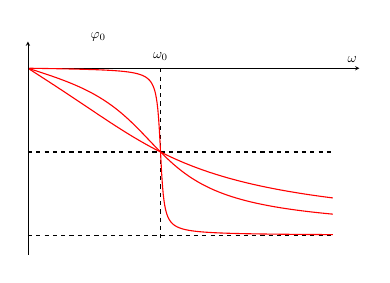
\begin{tikzpicture}[scale=0.5]
				\begin{axis}[
						axis lines=center, xlabel={$\omega$}, ylabel={$\varphi_0$},
						x label style={anchor=south west, at={(axis description cs:0.95,0.88)}},
						y label style={anchor=south east, at={(axis description cs:0.25,0.98)}},
						xmin=0, xmax=2.5, ymin=-3.5, ymax=0.5, ticks=none,
						width=10cm, height=7cm, samples=400
					]
					\draw[dashed, thick] (axis cs:0,-1.5708) -- (axis cs:2.3,-1.5708);
					\draw[dashed, thick] (axis cs:0,-3.1416) -- (axis cs:2.3,-3.1416);
					\draw[dashed, thick] (axis cs:1.0,0) -- (axis cs:1.0,-3.2);
					\node[left=2pt] at (axis cs:0,0) {$0$};
					\node[left=2pt] at (axis cs:0,-1.5708) {$-\pi/2$};
					\node[left=2pt] at (axis cs:0,-3.1416) {$-\pi$};
					\node[above=2pt] at (axis cs:1.0,0) {$\omega_0$};
					\addplot [red, thick, domain=0.01:2.3] {-atan2(2*0.02*x, 1 - x^2) * pi / 180};
					\addplot [red, thick, domain=0.01:2.3] {-atan2(2*0.4*x, 1 - x^2) * pi / 180};
					\addplot [red, thick, domain=0.01:2.3] {-atan2(2*0.8*x, 1 - x^2) * pi / 180};
				\end{axis}
			\end{tikzpicture}
		\end{column}
	\end{columns}
\end{frame}
% ===========================================================================

% ============================== Слайд ## ===================================
\begin{frame}{Резонансна крива}{}
	\begin{columns}
		\begin{column}{0.5\linewidth}\justifying\small
			При слабкому затуханні $\omega_m\approx\omega_0$:
			\begin{equation*}
				\tcbhighmath{
					V_{\max} \approx \frac{\omega_0}{2\gamma}\emf_0,
				}
				\qquad V_{\text{ст}} = \emf_0.
			\end{equation*}
			\begin{equation*}
				\tcbhighmath{
					\frac{V_{\max}}{V_{\text{ст}}} = \frac{\omega_0}{2\gamma} = Q.
				}
			\end{equation*}
			Ширина резонансу по рівню $1/\sqrt2$:
			\begin{equation*}
				\tcbhighmath{
					\Delta\omega = 2\gamma = \frac{\omega_0}{Q}.
				}
			\end{equation*}
			Чим вища добротність --- тим вужчий і вищий резонанс.
		\end{column}
		\begin{column}{0.5\linewidth}\centering
			\begin{tikzpicture}[scale=0.48]
				\begin{axis}[
						declare function={
								w0=1.0; gamma=0.15; Vst=0.6;
								V0(\w) = Vst / sqrt((w0^2 - \w^2)^2 + 4*(gamma^2)*(\w^2));
							},
						axis lines=center, xlabel={$\omega$}, ylabel={$V_0$},
						x label style={anchor=north west, at={(axis description cs:0.98,0.02)}},
						y label style={anchor=south east, at={(axis description cs:0.02,0.98)}},
						xmin=0, xmax=2.5, ymin=0, ymax=2.4, ticks=none,
						width=10cm, height=6.5cm, samples=500, clip=false,
					]
					\pgfmathsetmacro{\wres}{sqrt(w0^2 - 2*gamma^2)}
					\pgfmathsetmacro{\Vmax}{Vst / sqrt((w0^2 - \wres^2)^2 + 4*(gamma^2)*(\wres^2))}
					\draw[dashed, thick] (axis cs:0,\Vmax) -- (axis cs:\wres,\Vmax);
					\draw[thick] (axis cs:-0.03,\Vmax) -- (axis cs:0.03,\Vmax) node[left=3pt] {$V_{\max}$};
					\draw[thick] (axis cs:-0.03,{Vst}) -- (axis cs:0.03,{Vst}) node[left=3pt] {$V_{\text{ст}}$};
					\draw[thick] (axis cs:{w0},-0.04) -- (axis cs:{w0},0.04) node[below=3pt] {$\omega_0$};
					\addplot [red, thick, domain=0:2.3] {V0(x)};
				\end{axis}
			\end{tikzpicture}
		\end{column}
	\end{columns}
\end{frame}
% ===========================================================================

%% --------------------------------------------------------
\section{Змінний струм}
%% --------------------------------------------------------

% ============================== Слайд ## ===================================
\begin{frame}{Закон Ома в комплексній формі. Імпеданс}{}
	\begin{block}{}\justifying
		Із $\hat J_0 = i\omega C\hat V_0$ отримуємо \alert{закон Ома в комплексній формі}:
		\begin{equation*}
			\tcbhighmath{
				\hat J_0 Z = \emf_0, \qquad
				Z = R + i\left(\omega L - \frac1{\omega C}\right),
			}
		\end{equation*}
		де $Z$ --- \alert{імпеданс} (комплексний опір) кола.
	\end{block}
	\begin{block}{}\justifying
		Імпеданси елементів (для послідовного з'єднання $Z=Z_R+Z_L+Z_C$):
		\begin{equation*}
			Z_R = R, \qquad Z_L = i\omega L, \qquad Z_C = \frac1{i\omega C} = -\frac{i}{\omega C}.
		\end{equation*}
	\end{block}
	\begin{exampleblock}{}\justifying\small
		$\operatorname{Re}Z=R$ --- \alert{активний опір} (втрати енергії), $\operatorname{Im}Z=\omega L-1/\omega C$ --- \alert{реактивний опір} (без втрат). Напруга на $R$ --- у фазі зі струмом, на $C$ --- відстає на $\pi/2$, на $L$ --- випереджає на $\pi/2$.
	\end{exampleblock}
\end{frame}
% ===========================================================================

% ============================== Слайд ## ===================================
\begin{frame}{Векторні діаграми}{}
	\begin{columns}
		\begin{column}{0.48\linewidth}\justifying
			Комплексні амплітуди зображують векторами на комплексній площині; закон Ома $\hat J_0Z=\emf_0$ стає твердженням про їхню \alert{векторну суму}. Для $LCR$-контуру звідси відразу:
			\begin{equation*}
				\emf_0^2 = R^2J_0^2 + \left(\omega L - \frac1{\omega C}\right)^2 J_0^2.
			\end{equation*}
		\end{column}
		\begin{column}{0.52\linewidth}\centering
			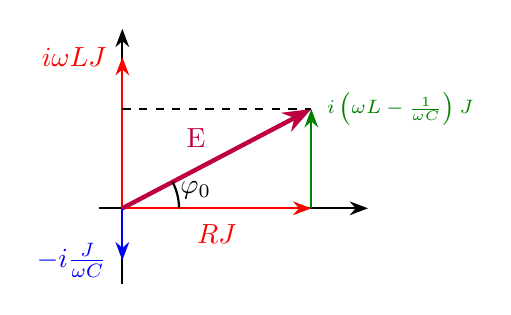
\begin{tikzpicture}[>=Stealth, line width=0.8pt, scale=0.6]
				\pgfmathsetmacro{\uR}{4.0}
				\pgfmathsetmacro{\uL}{3.2}
				\pgfmathsetmacro{\uC}{1.1}
				\pgfmathsetmacro{\uReac}{\uL - \uC}
				\pgfmathsetmacro{\phiDeg}{atan2(\uReac, \uR)}
				\coordinate (O2) at (0, 0);
				\coordinate (A) at (\uR, 0);
				\coordinate (UL_OY) at (0, \uL);
				\coordinate (UC_OY) at (0, -\uC);
				\coordinate (C) at (\uR, \uReac);
				\coordinate (U_reac) at (0, \uReac);
				\draw[->] (-0.5,0) -- (\uR + 1.2, 0);
				\draw[->] (0, -\uC - 0.5) -- (0, \uL + 0.6);
				\draw[red, ->, thick] (O2) -- (UL_OY) node[left=2pt] {$i\omega LJ$};
				\draw[blue, ->, thick] (O2) -- (UC_OY) node[left=2pt] {$-i\frac{J}{\omega C}$};
				\draw[red, ->, thick] (O2) -- (A) node[midway, below=2pt] {$RJ$};
				\draw[green!50!black, ->, thick] (A) -- (C) node[right=2pt] {\scriptsize $i\left(\omega L-\frac1{\omega C}\right)J$};
				\draw[purple, ->, ultra thick] (O2) -- (C) node[midway, above left] {$\emf$};
				\draw[dashed] (U_reac) -- (C);
				\draw (1.2, 0) arc (0:\phiDeg:1.2);
				\node at ({\phiDeg/2}:1.6) {$\varphi_0$};
			\end{tikzpicture}
		\end{column}
	\end{columns}
\end{frame}
% ===========================================================================

% ============================== Слайд ## ===================================
\begin{frame}{Потужність змінного струму}{}
	\begin{block}{}\justifying
		Середня за період потужність через комплексні амплітуди:
		\begin{equation*}
			\tcbhighmath{
				\overline Q = \frac12\operatorname{Re}\!\left[\hat\emf(t)\hat J^*(t)\right]
				= \frac12\emf_0J_0\cos\varphi_0.
			}
		\end{equation*}
	\end{block}
	\begin{block}{}\justifying
		З ефективними значеннями $J_{\text{eff}} = J_0/\sqrt2$, $\emf_{\text{eff}}=\emf_0/\sqrt2$:
		\begin{equation*}
			\tcbhighmath{
				\overline Q = \emf_{\text{eff}}J_{\text{eff}}\cos\varphi_0 = RJ_{\text{eff}}^2.
			}
		\end{equation*}
		За відсутності активного опору змінний струм роботи не виконує.
	\end{block}
	\begin{exampleblock}{}\justifying\small
		Втрати в лінії $\overline Q_{\text{втрат}}=RJ_{\text{eff}}^2$ залежать від струму, а не потужності --- тому електроенергію передають при високій напрузі й малому струмі (система Тесли--Вестінгауза, обрана 1893 р. замість постійнострумової мережі Едісона).
	\end{exampleblock}
\end{frame}
% ===========================================================================

% ============================== Слайд ## ===================================
\begin{frame}{Резонанс напруг}{}
	\begin{columns}
		\begin{column}{0.5\linewidth}\justifying\small
			У послідовному $LCR$-контурі на частоті $\omega_0=1/\sqrt{LC}$ маємо $Z_L+Z_C=0$, тож $J_0(\omega)$ максимальний:
			\begin{equation*}
				\tcbhighmath{
					J_{0,\max} = \frac{\emf_0}{R}.
				}
			\end{equation*}
			Напруга на конденсаторі (і котушці) в резонансі:
			\begin{equation*}
				\tcbhighmath{
					V_{C,\max} = Q\,\emf_0.
				}
			\end{equation*}
		\end{column}
		\begin{column}{0.5\linewidth}\centering
			\begin{tikzpicture}[scale=0.5]
				\begin{axis}[
						declare function={ L=1.0; C=1.0; R=0.25; E0=1.0; w0=1.0/sqrt(L*C);
								J0(\w) = E0 / sqrt(R^2 + (\w*L - 1/(\w*C))^2); },
						axis lines=center, xlabel={$\omega$}, ylabel={$J_0$},
						x label style={anchor=north west, at={(axis description cs:0.98,0.02)}},
						y label style={anchor=south east, at={(axis description cs:0.02,0.98)}},
						xmin=0, xmax=2.5, ymin=0, ymax=4.5, xtick=\empty, ytick=\empty,
						extra x ticks={1.0}, extra x tick labels={$\omega_0$},
						width=9cm, height=6.5cm, samples=600, clip=false,
					]
					\addplot [red, thick, domain=0.05:2.4] {J0(x)};
				\end{axis}
			\end{tikzpicture}
		\end{column}
	\end{columns}
	\begin{alertblock}{}\justifying\small
		Кожна з напруг (на $L$ і на $C$) окремо в $Q$ разів перевищує напругу джерела --- при $Q\sim100$ і $220$ В це вже $22$ кВ (\alert{перенапруга}). У радіотехніці ж це використовують для підсилення слабкого сигналу.
	\end{alertblock}
\end{frame}
% ===========================================================================

% ============================== Слайд ## ===================================
\begin{frame}{Резонанс струмів}{}
	\begin{columns}
		\begin{column}{0.46\linewidth}
			\begin{circuitikz}[european resistors, scale=0.75, thick]
				\coordinate (L0) at (0, 0);
				\coordinate (L1) at (0, 1.0);
				\coordinate (L2) at (0, 2.0);
				\coordinate (L3) at (0, 3.0);
				\coordinate (R0) at (3, 0);
				\coordinate (R1) at (3, 1.0);
				\coordinate (R2) at (3, 2.0);
				\coordinate (R3) at (3, 3.0);
				\draw (L3) to[L, l=$L$] (R3);
				\draw (L2) to[C, l=$C$] (R2);
				\draw (L1) to[R, l=$R$] (R1);
				\draw (L0) to[isourcesin, l_=$J(t)$] (R0);
				\draw (L0) -- (L3);
				\draw (R0) -- (R3);
			\end{circuitikz}
		\end{column}
		\begin{column}{0.54\linewidth}\justifying\small
			Паралельний $LCR$-контур із джерелом струму: $J=J_R+J_L+J_C$. На $\omega_0$ блок $L\parallel C$ має нескінченний опір, тож
			\begin{equation*}
				(J_{R0})_{\max} = J_0, \qquad
				\tcbhighmath{
					J_{L0} = J_{C0} = \frac{J_0}{Q},
				}
			\end{equation*}
			де добротність паралельного контуру $Q=R\sqrt{C/L}$ (для послідовного --- $Q=\frac1R\sqrt{L/C}$).
		\end{column}
	\end{columns}
	\begin{exampleblock}{}\justifying\small
		Якщо джерело --- ЕРС, на $\omega_0$ був би \alert{мінімум} струму (\alert{антирезонанс}). Ефект резонансу струмів використовують в індукційних печах і плитах: струм у котушці зростає в багато разів при відносно малому струмі підводу.
	\end{exampleblock}
\end{frame}
% ===========================================================================

% ============================== Слайд ## ===================================
\begin{frame}{Правила Кірхгофа для змінного струму}{}
	\begin{block}{}\justifying
		Ті самі правила, що й для постійного струму, з заміною $R\to Z$:
	\end{block}
	\begin{exampleblock}{}\justifying
		\textbf{1.} Сума струмів, що входять у вузол:
		\begin{equation*}
			\tcbhighmath{
				\sum_k J_k = 0
			}
		\end{equation*}
		--- наслідок закону збереження заряду.
	\end{exampleblock}
	\begin{exampleblock}{}\justifying
		\textbf{2.} Для будь-якого замкнутого контуру:
		\begin{equation*}
			\tcbhighmath{
				\sum_k J_kZ_k = \sum_i \emf_i
			}
		\end{equation*}
		--- наслідок закону індукції (теореми про циркуляцію).
	\end{exampleblock}
\end{frame}
% ===========================================================================

% ============================== Слайд ## ===================================
\begin{frame}{Приклад: розгалужене коло}{}
	\begin{columns}
		\begin{column}{0.42\linewidth}
			\begin{circuitikz}[european resistors, scale=0.75, thick]
				\coordinate (A) at (0,0);
				\coordinate (B) at (2.5,0);
				\coordinate (C) at (5,0);
				\coordinate (D) at (0,2.5);
				\coordinate (E) at (2.5,2.5);
				\coordinate (F) at (5,2.5);
				\draw (D) to[isourcesin, l=$\emf$] (A);
				\draw (D) to[L, l_=$L$] (E);
				\draw (E) to[R, l_=$R$] (B);
				\draw (E) to[C, l_=$C$] (F);
				\draw (B) -- (A);
				\draw (F) -- (C);
				\draw (B) -- (C);
				\fill (E) circle (2.5pt);
			\end{circuitikz}
		\end{column}
		\begin{column}{0.58\linewidth}\justifying\small
			Котушка $L$ послідовно з паралельно з'єднаними $R$ і $C$. Перше правило Кірхгофа у вузлі: $J=J_R+J_C$. Друге --- для двох контурів: $Z_LJ+RJ_R=\emf$, $Z_LJ+Z_CJ_C=\emf$.
		\end{column}
	\end{columns}
	\begin{block}{}\justifying
		Розв'язуючи систему, повний імпеданс кола:
		\begin{equation*}
			\tcbhighmath{
				Z = Z_L + Z_{RC}, \qquad
				Z_{RC} = \frac{R}{1+i\omega RC}.
			}
		\end{equation*}
		Диференціальне рівняння звелося до системи \alert{лінійних алгебраїчних} рівнянь із комплексними коефіцієнтами --- у цьому і полягає сила методу комплексних амплітуд.
	\end{block}
\end{frame}
% ===========================================================================

% ============================== Слайд ## ===================================
\begin{frame}{Фільтр низьких частот (ФНЧ)}{}
	\begin{columns}
		\begin{column}{0.46\linewidth}
			\begin{circuitikz}[european resistors, scale=0.8, thick]
				\coordinate (A) at (0,0);
				\coordinate (B) at (3,0);
				\coordinate (C) at (3,2);
				\coordinate (D) at (0,2);
				\draw (D) to[R, l=$R$] (C);
				\draw (C) to[C, l_=$C$] (B);
				\draw (A) -- (B);
				\draw (D) to[short, -o] ($(D)!0.3!(A)$);
				\draw (A) to[short, -o] ($(D)!0.7!(A)$);
				\draw (C) to[short, -o] ($(C)!0.3!(B)$);
				\draw (B) to[short, -o] ($(C)!0.7!(B)$);
			\end{circuitikz}
		\end{column}
		\begin{column}{0.54\linewidth}\justifying\small
			Вихідна напруга --- з конденсатора:
			\begin{equation*}
				\tcbhighmath{
					K(\omega) = \frac{U_{\text{вих}}}{U_{\text{вх}}} = \frac1{1+i\omega RC}.
				}
			\end{equation*}
			$|K|\to1$ на низьких, $|K|\to0$ на високих частотах; гранична частота $\omega_c=1/RC$.
		\end{column}
	\end{columns}
	\begin{exampleblock}{}\justifying\small
		Застосування: згладжування пульсацій у випрямлячах живлення.
	\end{exampleblock}
\end{frame}
% ===========================================================================

% ============================== Слайд ## ===================================
\begin{frame}{Фільтр високих частот (ФВЧ)}{}
	\begin{columns}
		\begin{column}{0.46\linewidth}
			\begin{circuitikz}[european resistors, scale=0.8, thick]
				\coordinate (A) at (0,0);
				\coordinate (B) at (3,0);
				\coordinate (C) at (3,2);
				\coordinate (D) at (0,2);
				\draw (D) to[C, l=$C$] (C);
				\draw (C) to[R, l_=$R$] (B);
				\draw (A) -- (B);
			\end{circuitikz}
		\end{column}
		\begin{column}{0.54\linewidth}\justifying\small
			Вихідна напруга --- з резистора:
			\begin{equation*}
				\tcbhighmath{
					K(\omega) = \frac{i\omega RC}{1+i\omega RC}.
				}
			\end{equation*}
			$|K|\to0$ на низьких, $|K|\to1$ на високих частотах.
		\end{column}
	\end{columns}
	\begin{exampleblock}{}\justifying\small
		Застосування: підключення твітера в акустичній системі (не пропускає низькі частоти).
	\end{exampleblock}
\end{frame}
% ===========================================================================

% ============================== Слайд ## ===================================
\begin{frame}{Смуговий фільтр}{}
	\begin{block}{}\justifying
		Послідовний $LCR$-контур, вихідна напруга --- з резистора:
		\begin{equation*}
			\tcbhighmath{
				K(\omega) = \frac1{1+iQ\left(\dfrac\omega{\omega_0} - \dfrac{\omega_0}\omega\right)},
			}
		\end{equation*}
		де $Q=\omega_0L/R$. Максимум $|K|=1$ при $\omega_0$, ширина смуги $\Delta\omega=\omega_0/Q$.
	\end{block}
	\begin{columns}
		\begin{column}{0.5\linewidth}\centering
			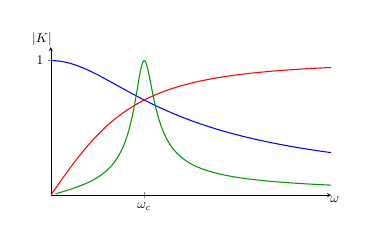
\begin{tikzpicture}[scale=0.48]
				\begin{axis}[
						declare function={ RC=1.0; wc=1.0/RC; KLP(\w)=1/sqrt(1+(\w*RC)^2);
								KHP(\w)=(\w*RC)/sqrt(1+(\w*RC)^2); Q=5.0; w0=1.0;
								KBP(\w)=1/sqrt(1+Q^2*(\w/w0-w0/\w)^2); },
						axis lines=center, xlabel={$\omega$}, ylabel={$|K|$},
						x label style={anchor=north west, at={(axis description cs:0.98,0.02)}},
						y label style={anchor=south east, at={(axis description cs:0.02,0.98)}},
						xmin=0, xmax=3, ymin=0, ymax=1.1, xtick={1}, xticklabels={$\omega_c$},
						ytick={1}, yticklabels={$1$}, width=9cm, height=5.5cm, samples=400,
					]
					\addplot [blue, thick, domain=0:3] {KLP(x)};
					\addplot [red, thick, domain=0:3] {KHP(x)};
					\addplot [green!60!black, thick, domain=0.05:3] {KBP(x)};
				\end{axis}
			\end{tikzpicture}
		\end{column}
		\begin{column}{0.5\linewidth}\justifying\small
			ФНЧ (синій), ФВЧ (червоний), смуговий (зелений, $Q=5$): реактивний опір залежить від частоти --- саме це визначає, які частоти пройдуть.
		\end{column}
	\end{columns}
\end{frame}
% ===========================================================================

% ============================== Слайд ## ===================================
\begin{frame}{Підсумки}{}
\begin{tblr}{
colspec={Q[c,l]Q[mode=dmath]}
}
Рівняння коливального контуру & L\dot J + JR + \frac qC = \emf \\
Рівняння вільних коливань & \ddot q + 2\gamma\dot q + \omega_0^2 q = 0,\ \ 2\gamma=\frac RL,\ \omega_0^2=\frac1{LC} \\
Формула Томсона & T = 2\pi\sqrt{LC} \\
Логарифмічний декремент & \delta = \gamma T \\
Добротність (посл. контур) & Q = \frac1R\sqrt{\frac LC} \\
Резонансна частота & \omega_m = \sqrt{\omega_0^2 - 2\gamma^2} \\
Ширина резонансу & \Delta\omega = \omega_0/Q \\
Імпеданс & Z = R + i\left(\omega L - \frac1{\omega C}\right) \\
Закон Ома (комплексний) & \hat J_0 Z = \emf_0 \\
Середня потужність & \overline Q = \emf_{\text{eff}}J_{\text{eff}}\cos\varphi_0 \\
Правила Кірхгофа & \sum_k J_k = 0,\quad \sum_k J_kZ_k=\sum_i\emf_i \\
Добротність (парал. контур) & Q = R\sqrt{\frac CL}
\end{tblr}
\end{frame}
% ===========================================================================

\end{document}
